\begin{figure}[H]
\centering
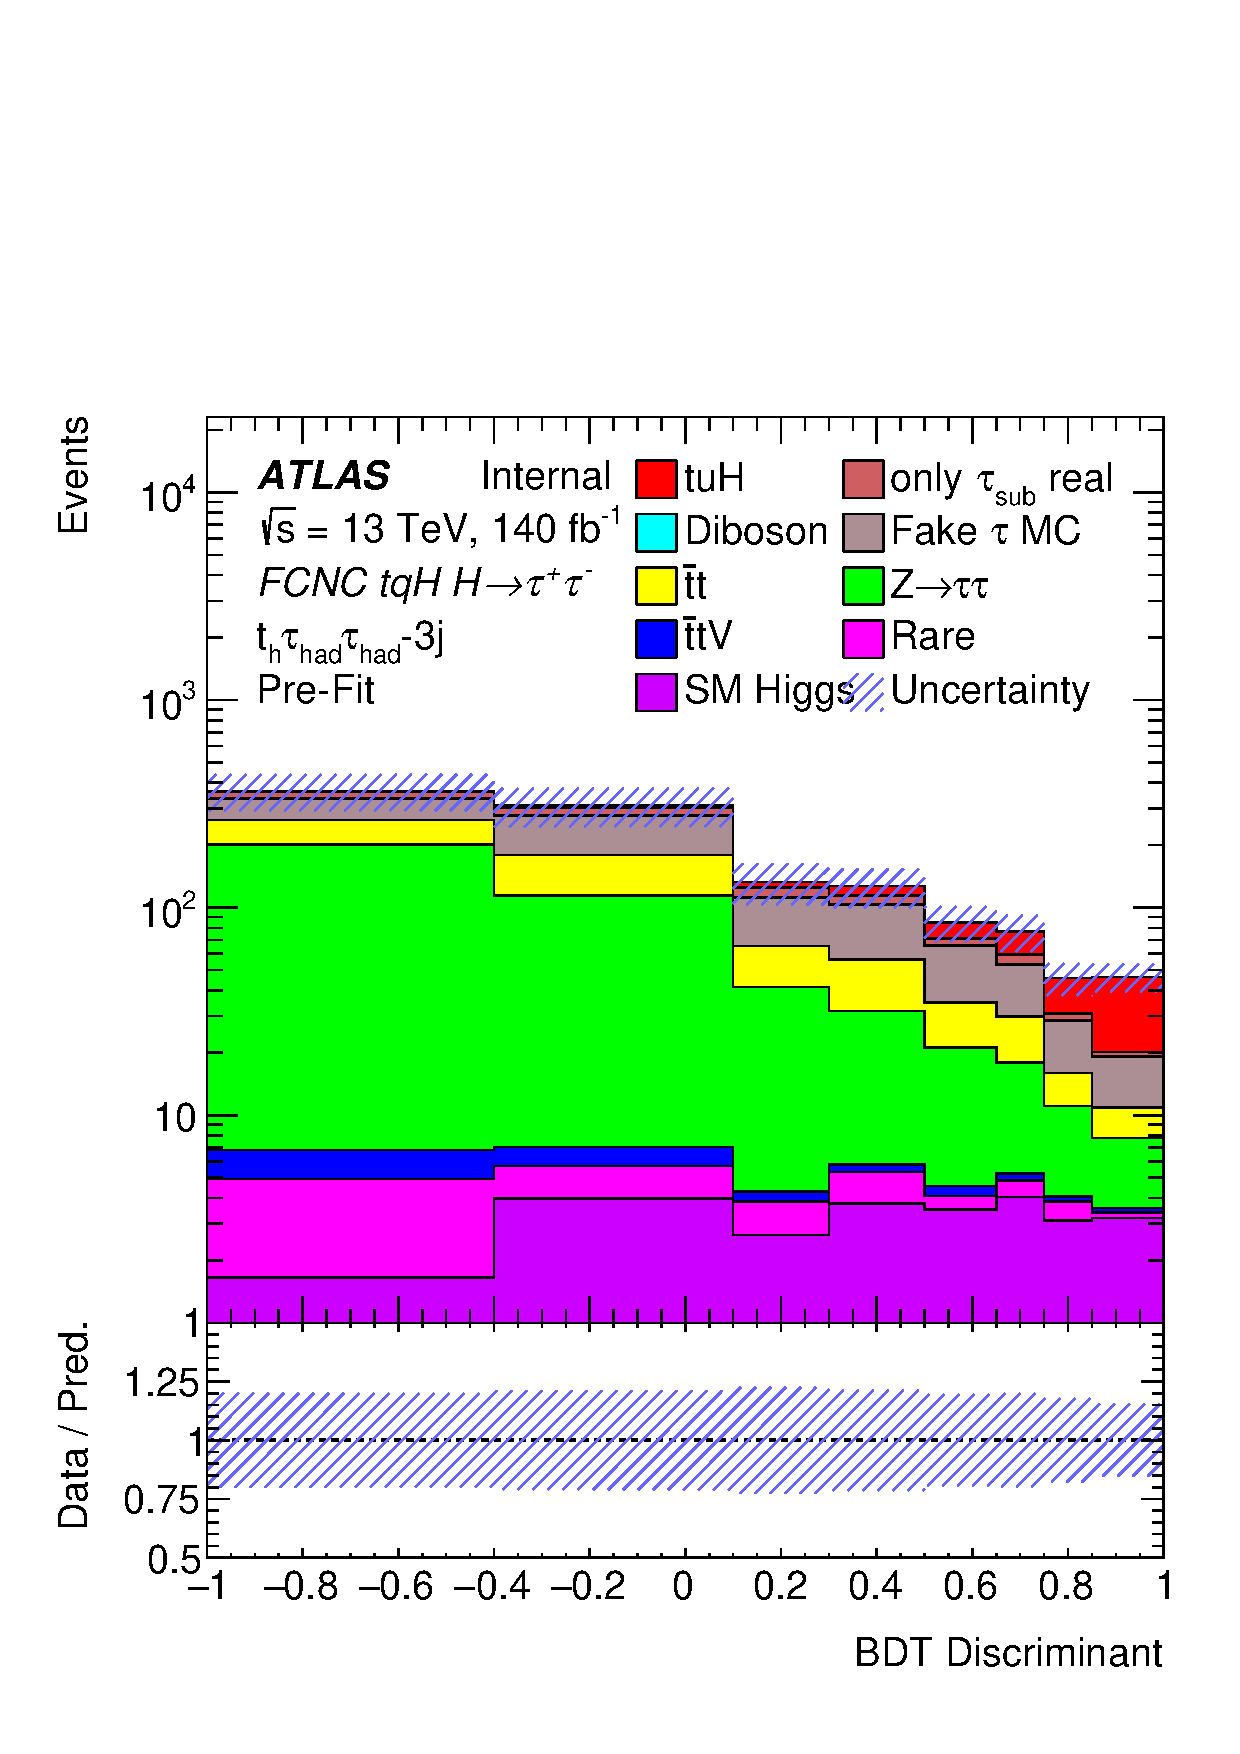
\includegraphics[width=0.30\textwidth]{\FCNCFigures/unblinded/xTFW/tuH_reg2mtau1b3jos_vetobtagwp70_highmet.pdf}
\put(-100, 55){\textbf{(a1)}}
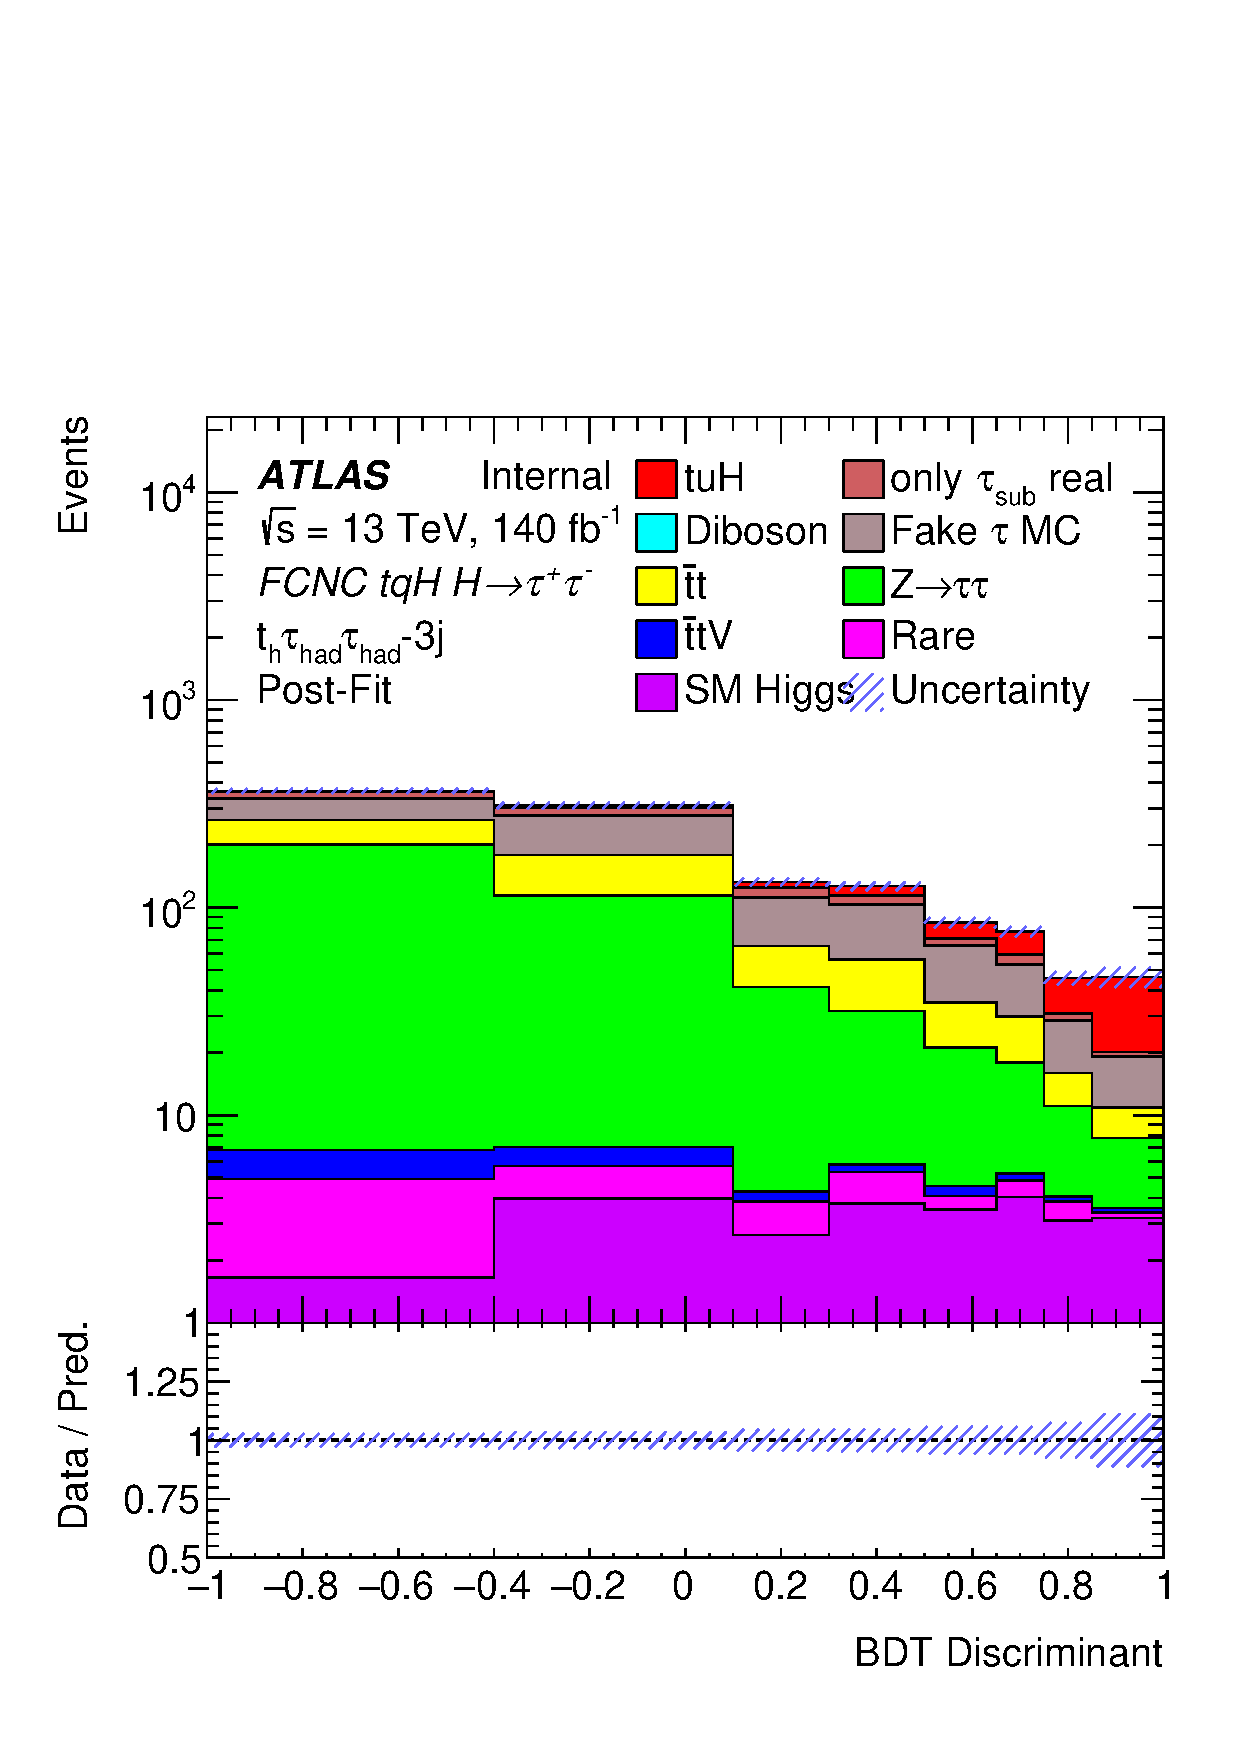
\includegraphics[width=0.30\textwidth]{\FCNCFigures/unblinded/xTFW/tuH_reg2mtau1b3jos_vetobtagwp70_highmet_postFit.pdf}
\put(-100, 55){\textbf{(a2)}}
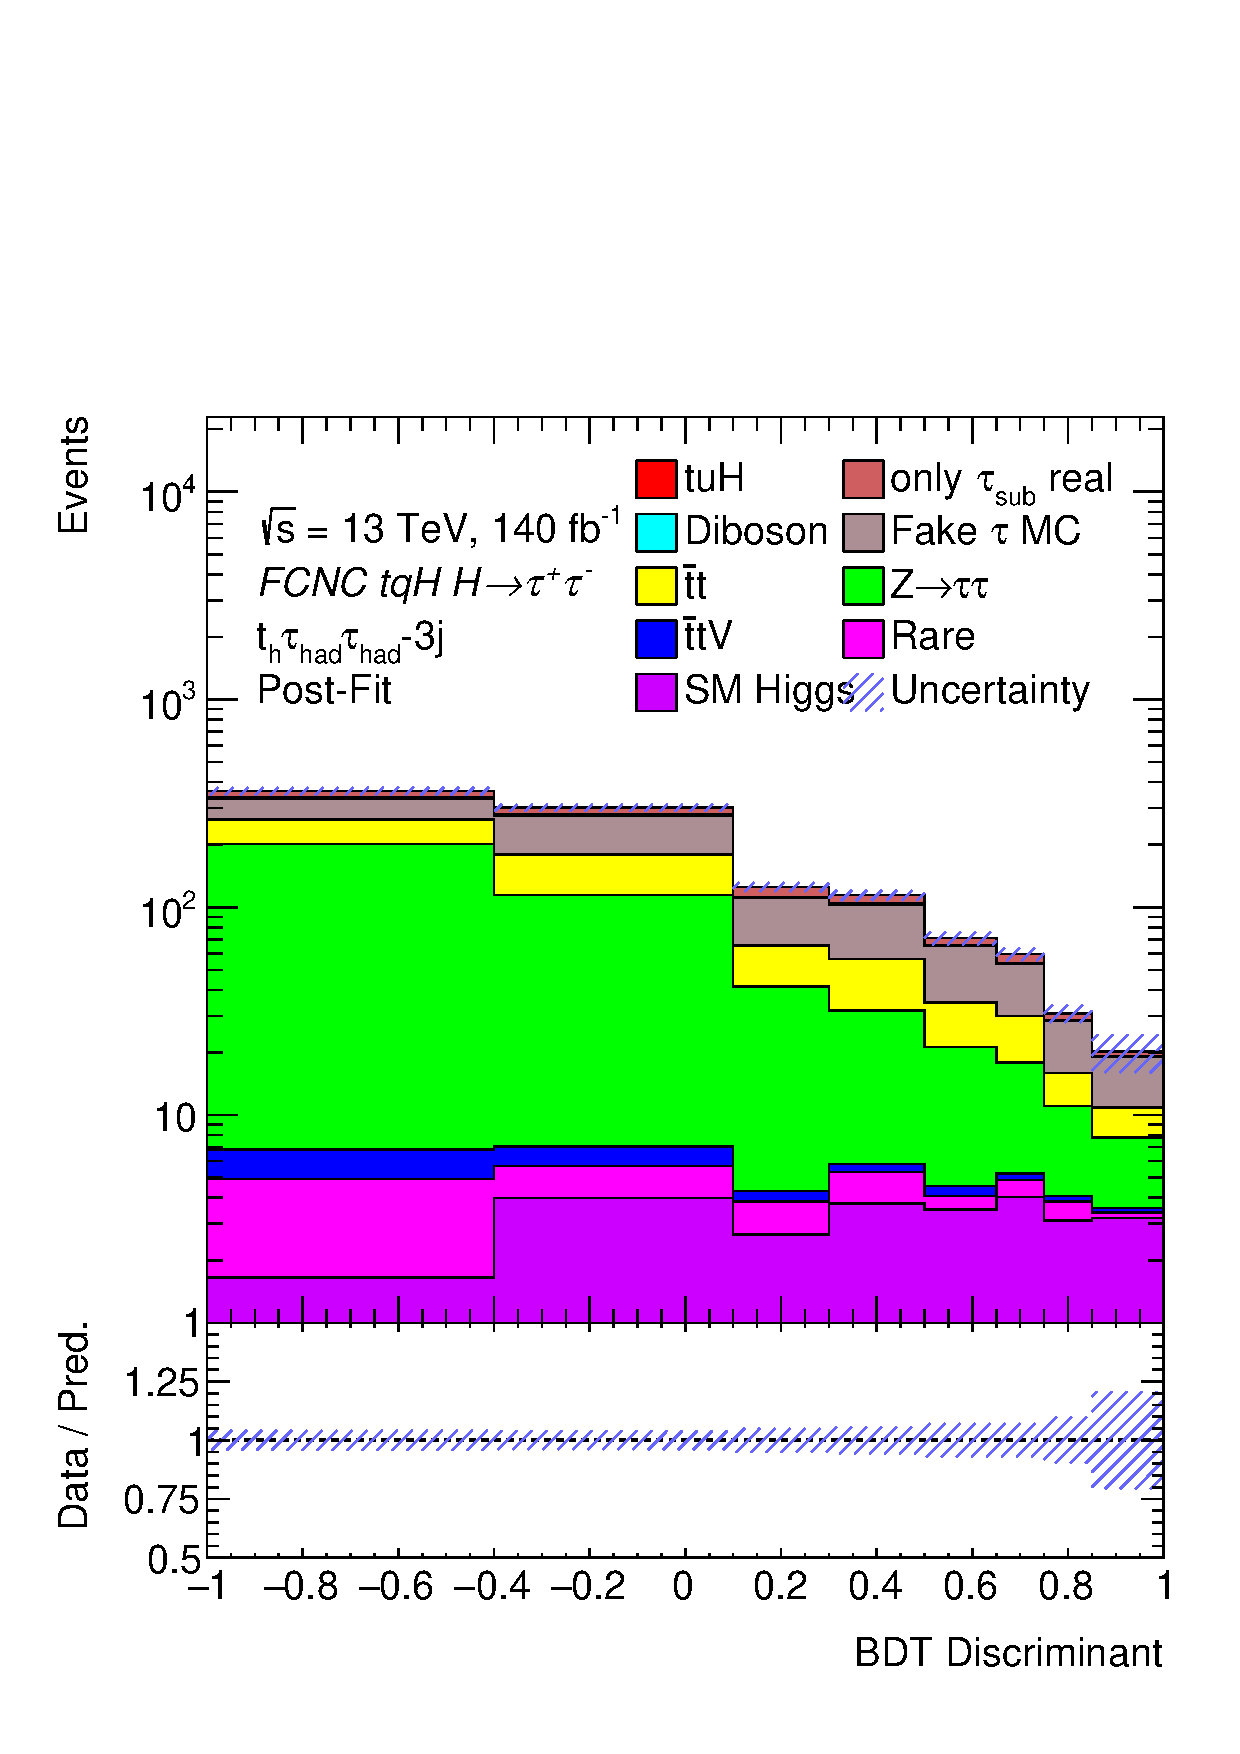
\includegraphics[width=0.30\textwidth]{\FCNCFigures/unblinded/xTFW/tuH_reg2mtau1b3jos_vetobtagwp70_highmet_postFit_BOnly.pdf}
\put(-100, 55){\textbf{(a3)}}\\
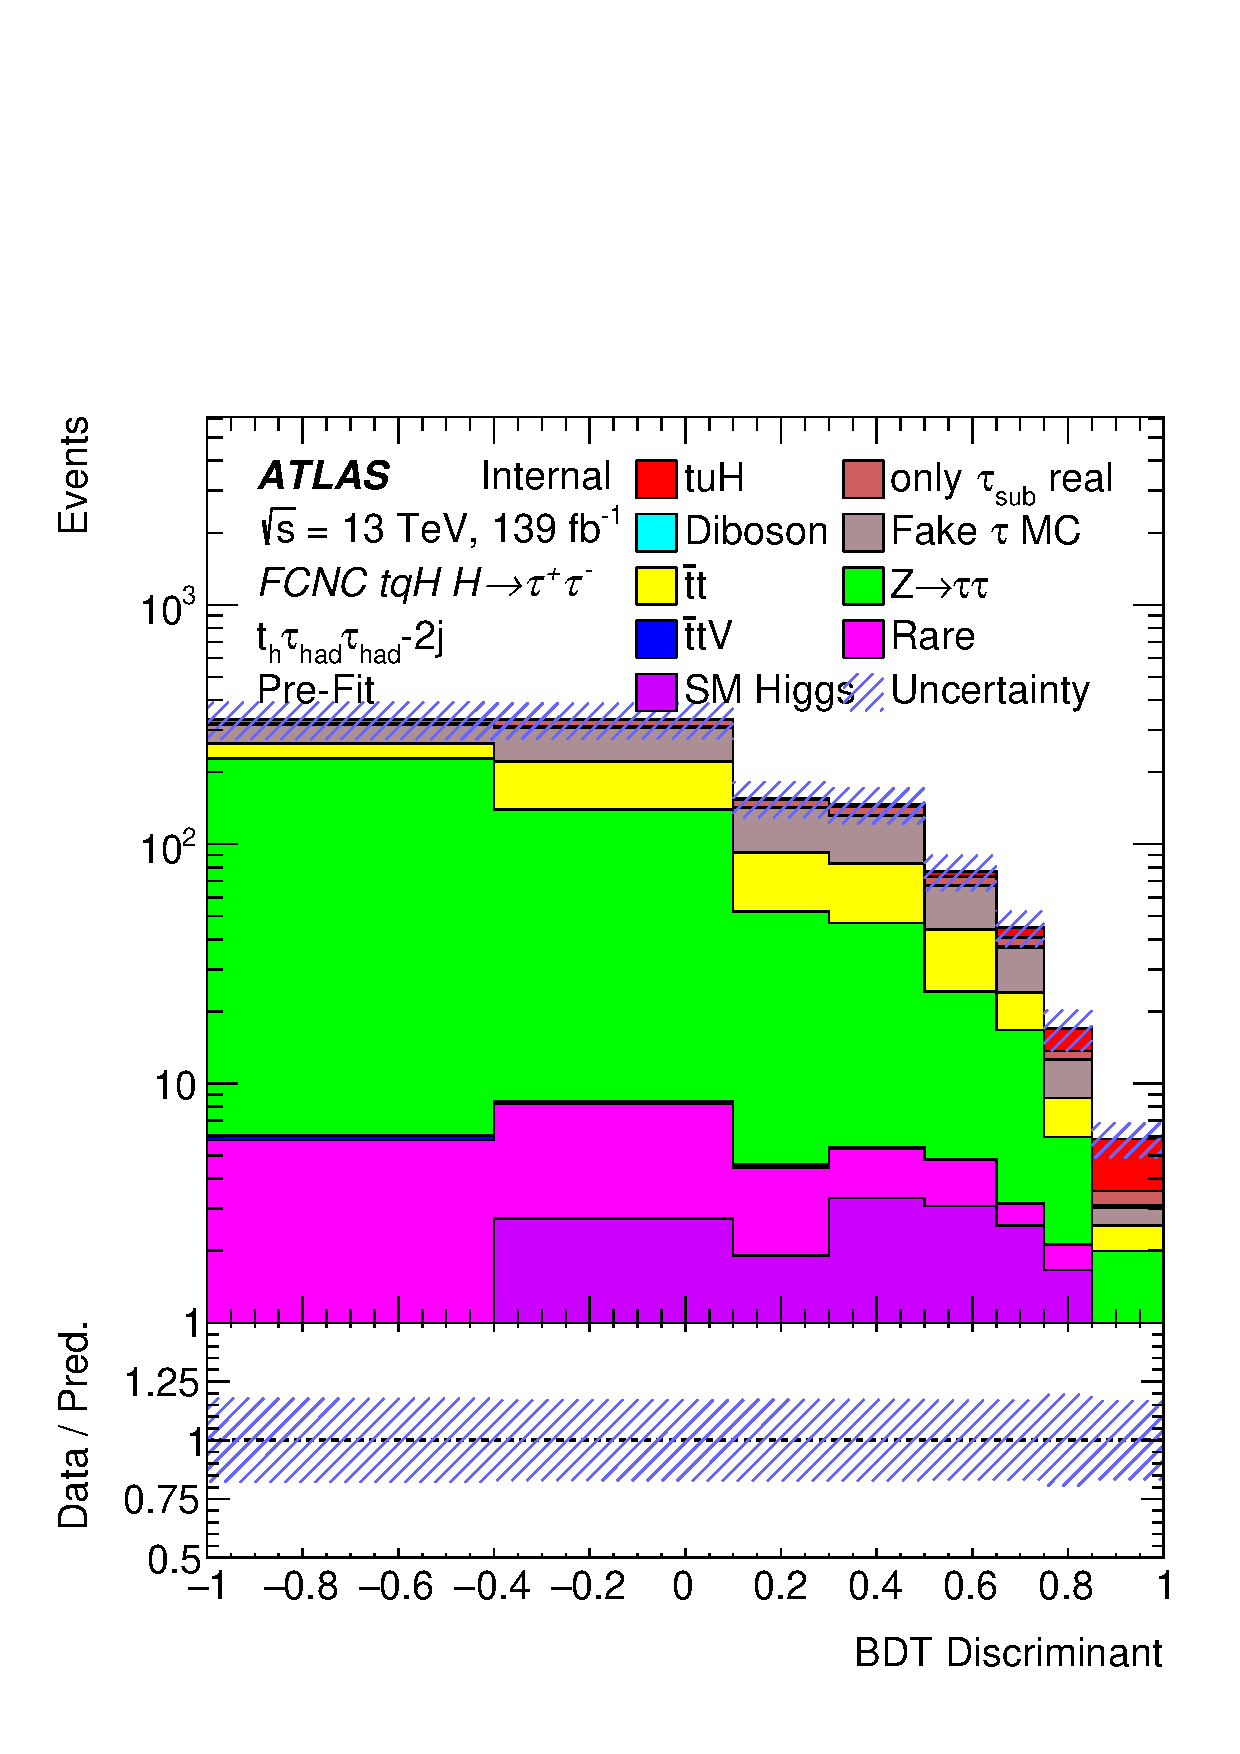
\includegraphics[width=0.30\textwidth]{\FCNCFigures/unblinded/xTFW/tuH_reg2mtau1b2jos_vetobtagwp70_highmet.pdf}
\put(-100, 55){\textbf{(b1)}}
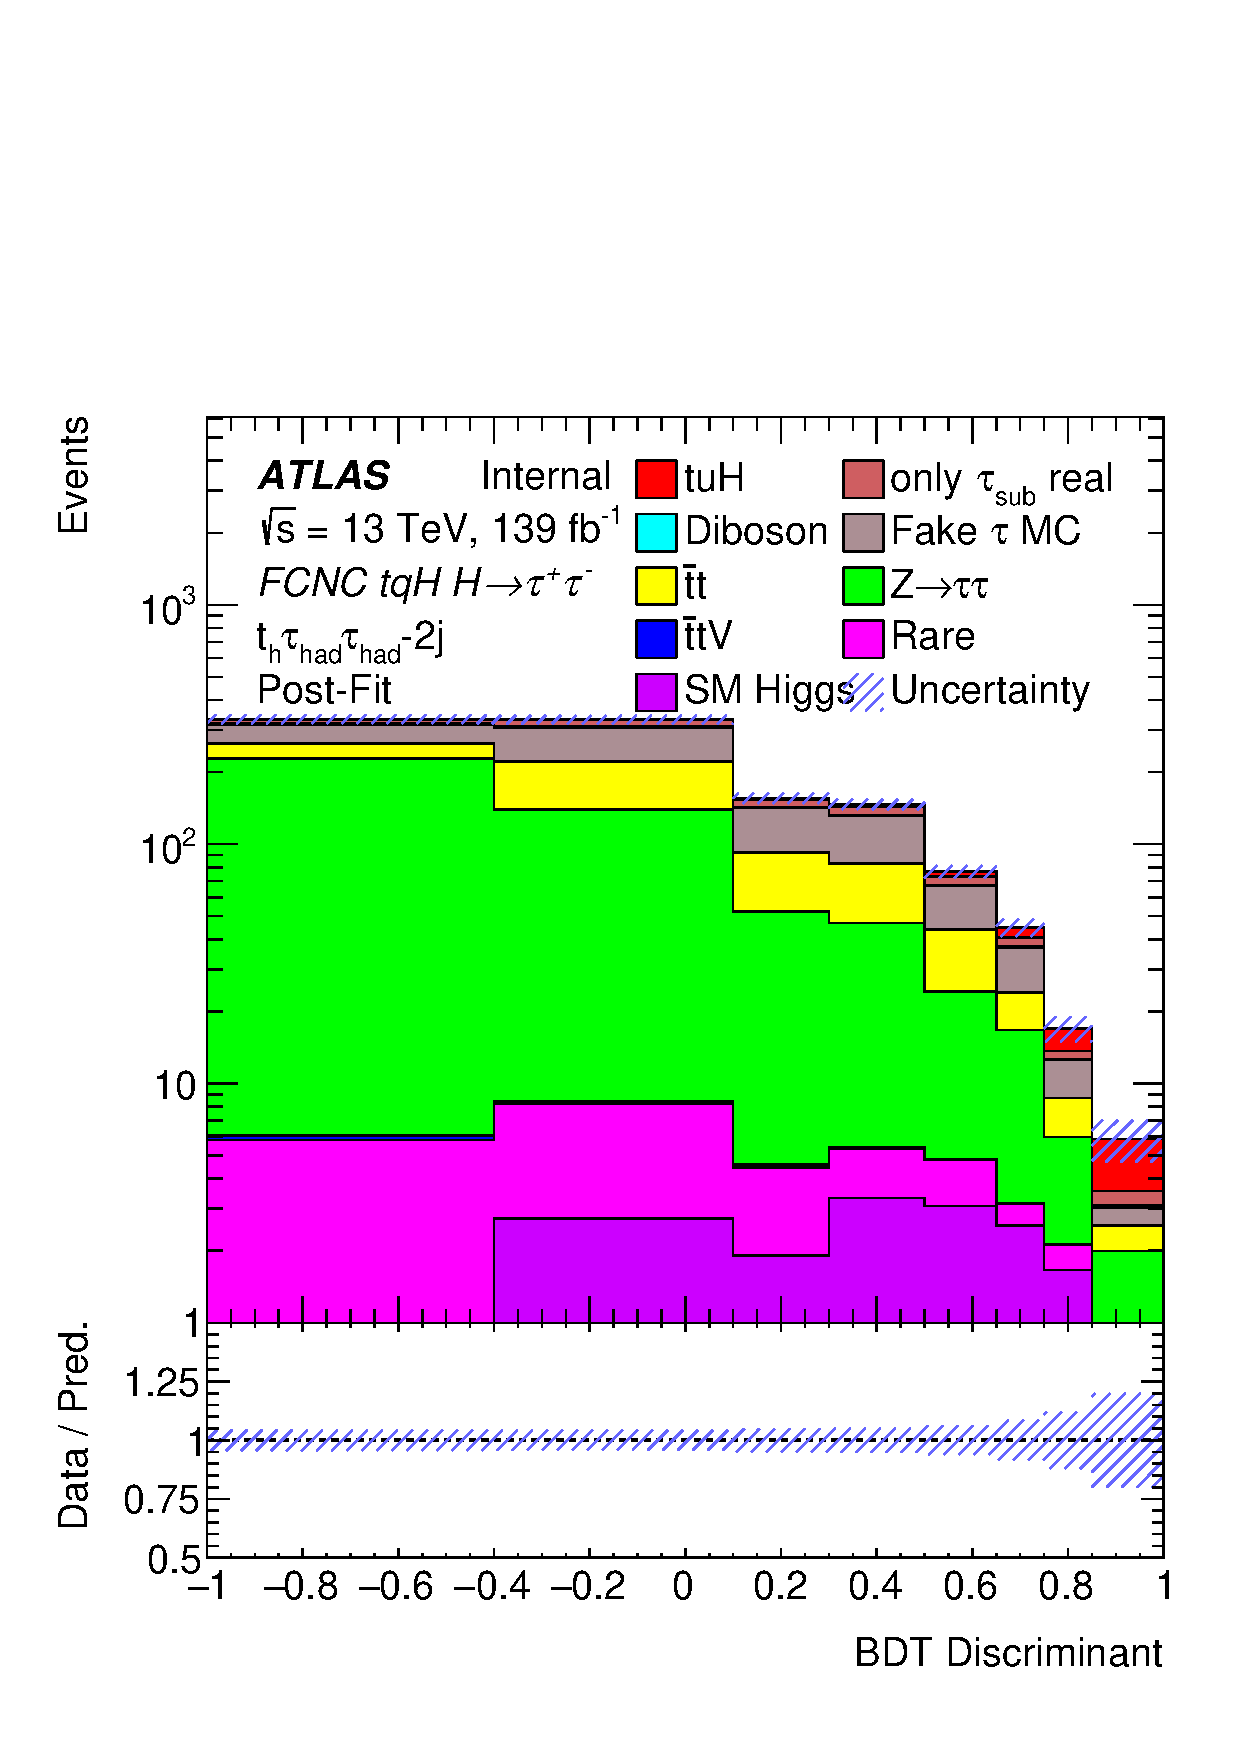
\includegraphics[width=0.30\textwidth]{\FCNCFigures/unblinded/xTFW/tuH_reg2mtau1b2jos_vetobtagwp70_highmet_postFit.pdf}
\put(-100, 55){\textbf{(b2)}}
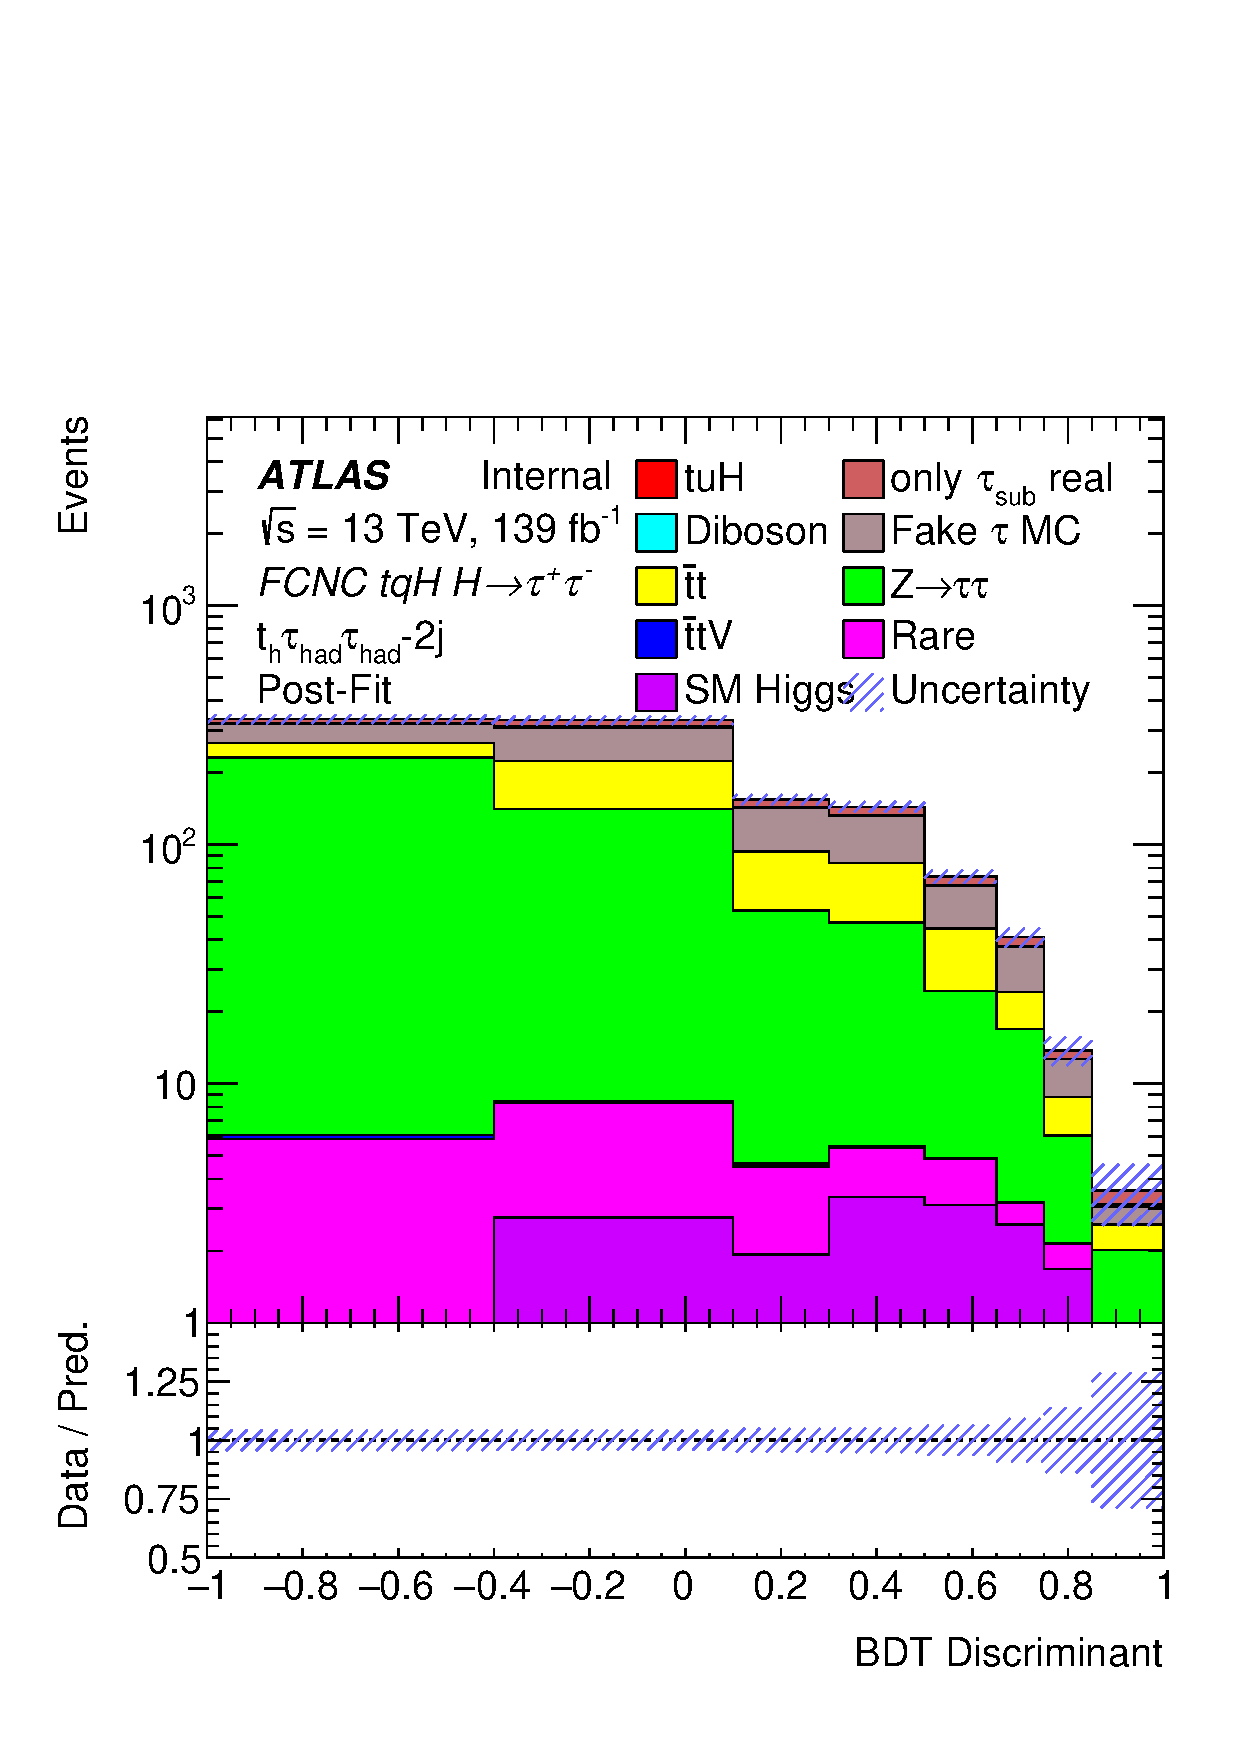
\includegraphics[width=0.30\textwidth]{\FCNCFigures/unblinded/xTFW/tuH_reg2mtau1b2jos_vetobtagwp70_highmet_postFit_BOnly.pdf}
\put(-100, 55){\textbf{(b3)}}\\

\caption{ Comparison of the shape of the BDT discriminant distribution between the unblinded prefit (a1,b1), unblinded postfit (a2,b2) and background only fit (a3,b3) in terms of tuH merged signal. The upper three plots are in the  $t_h\thadhad$-3j (a1-a3) region, and the bottom three are in $t_h\thadhad$-2j (b1-b3). Statistical and systematic uncertainties are being shown.}
\label{fig:xTFW_trexPrefit}
\end{figure}


\begin{figure}[H]
\centering
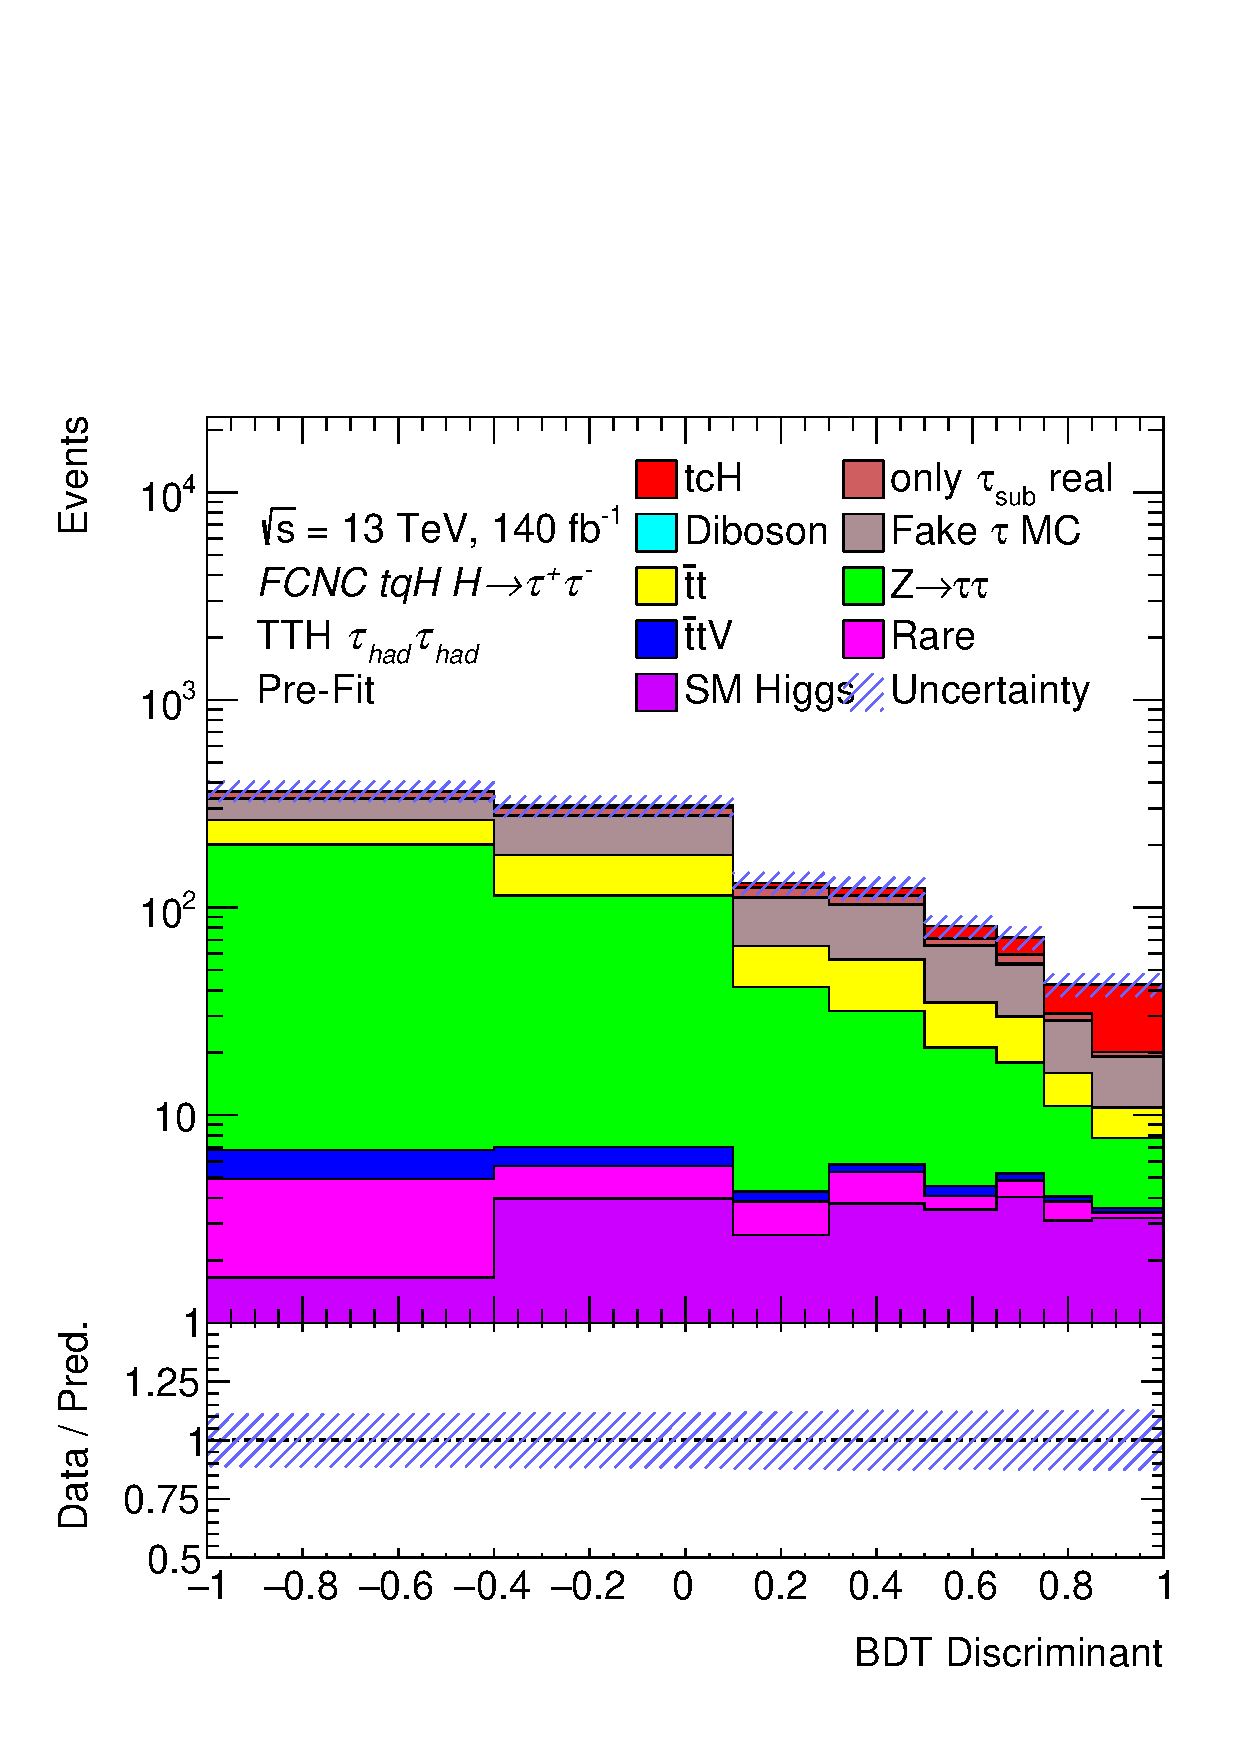
\includegraphics[width=0.30\textwidth]{\FCNCFigures/unblinded/xTFW/tcH_reg2mtau1b3jos_vetobtagwp70_highmet.pdf}
\put(-100, 55){\textbf{(a1)}}
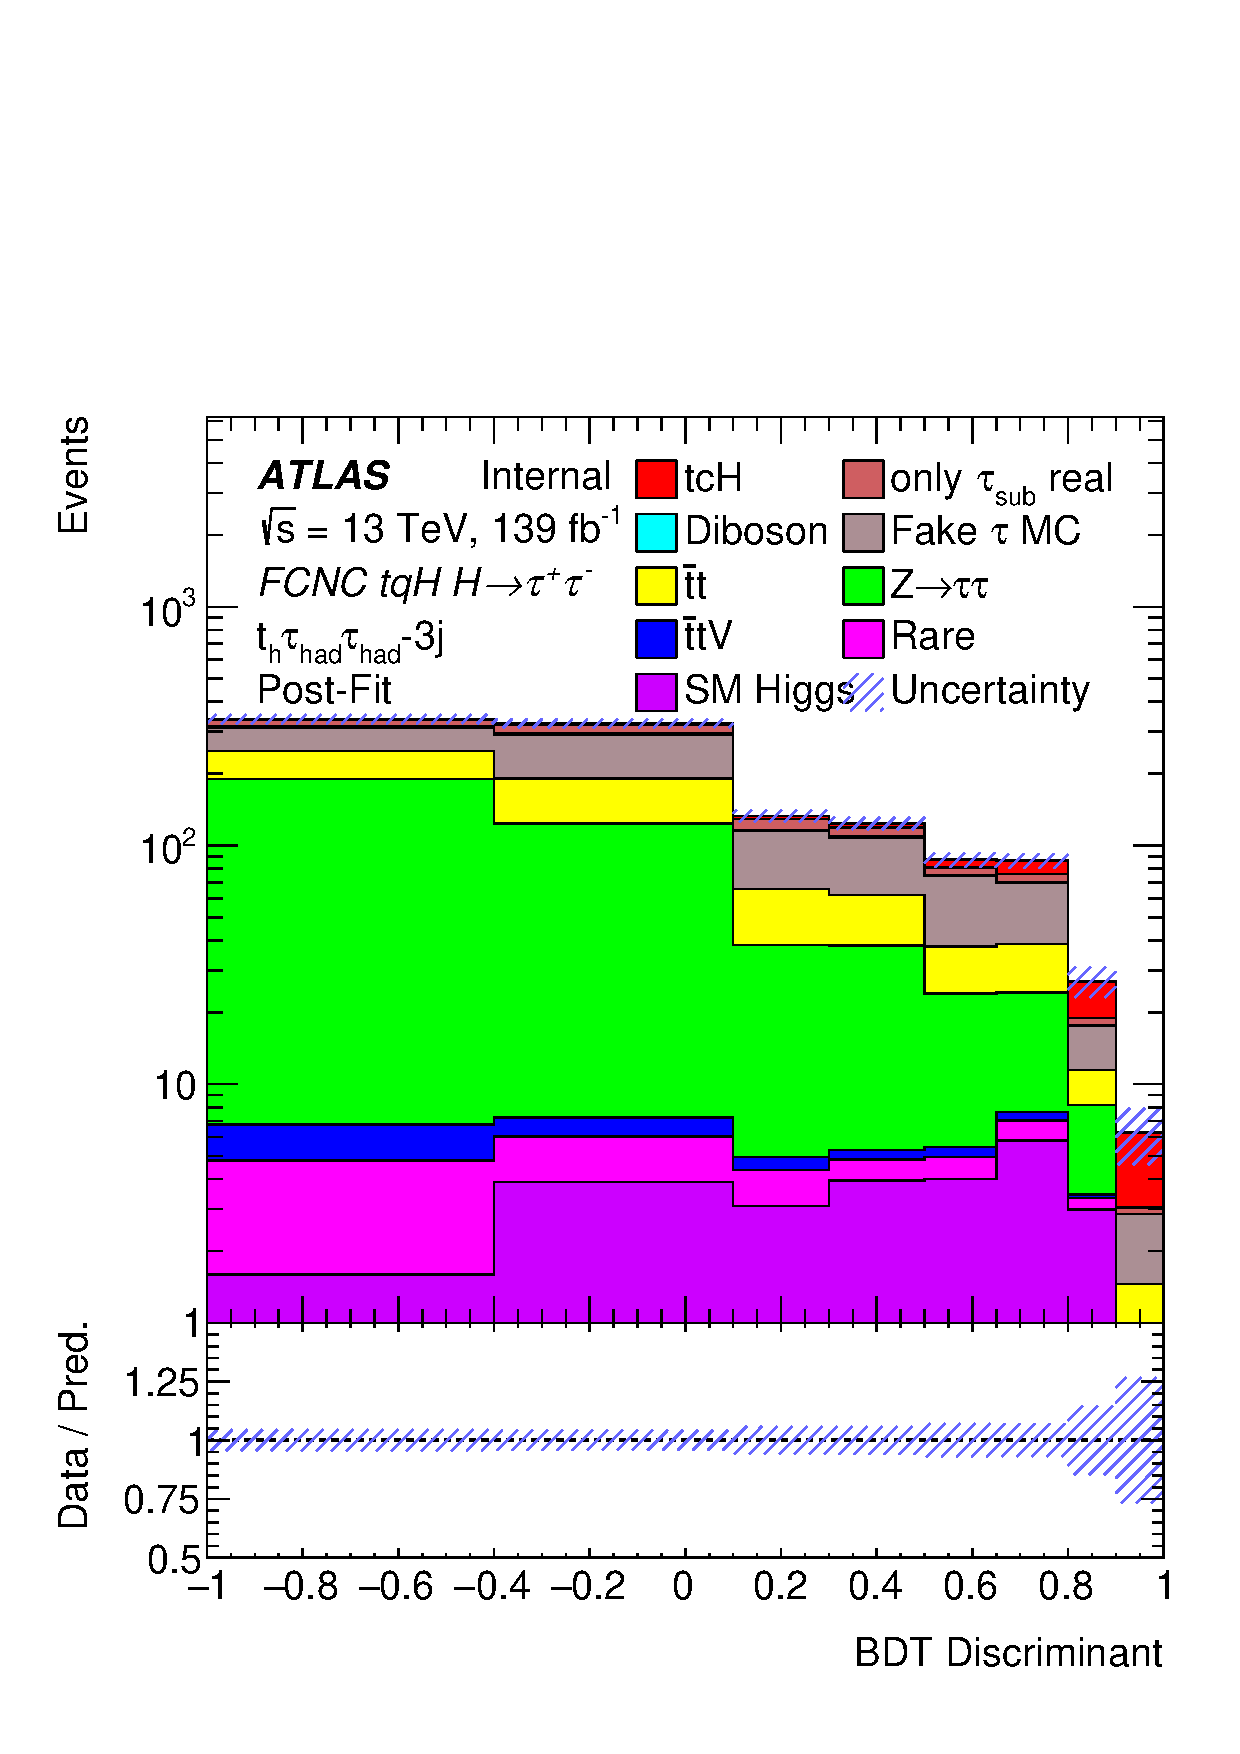
\includegraphics[width=0.30\textwidth]{\FCNCFigures/unblinded/xTFW/tcH_reg2mtau1b3jos_vetobtagwp70_highmet_postFit.pdf}
\put(-100, 55){\textbf{(a2)}}
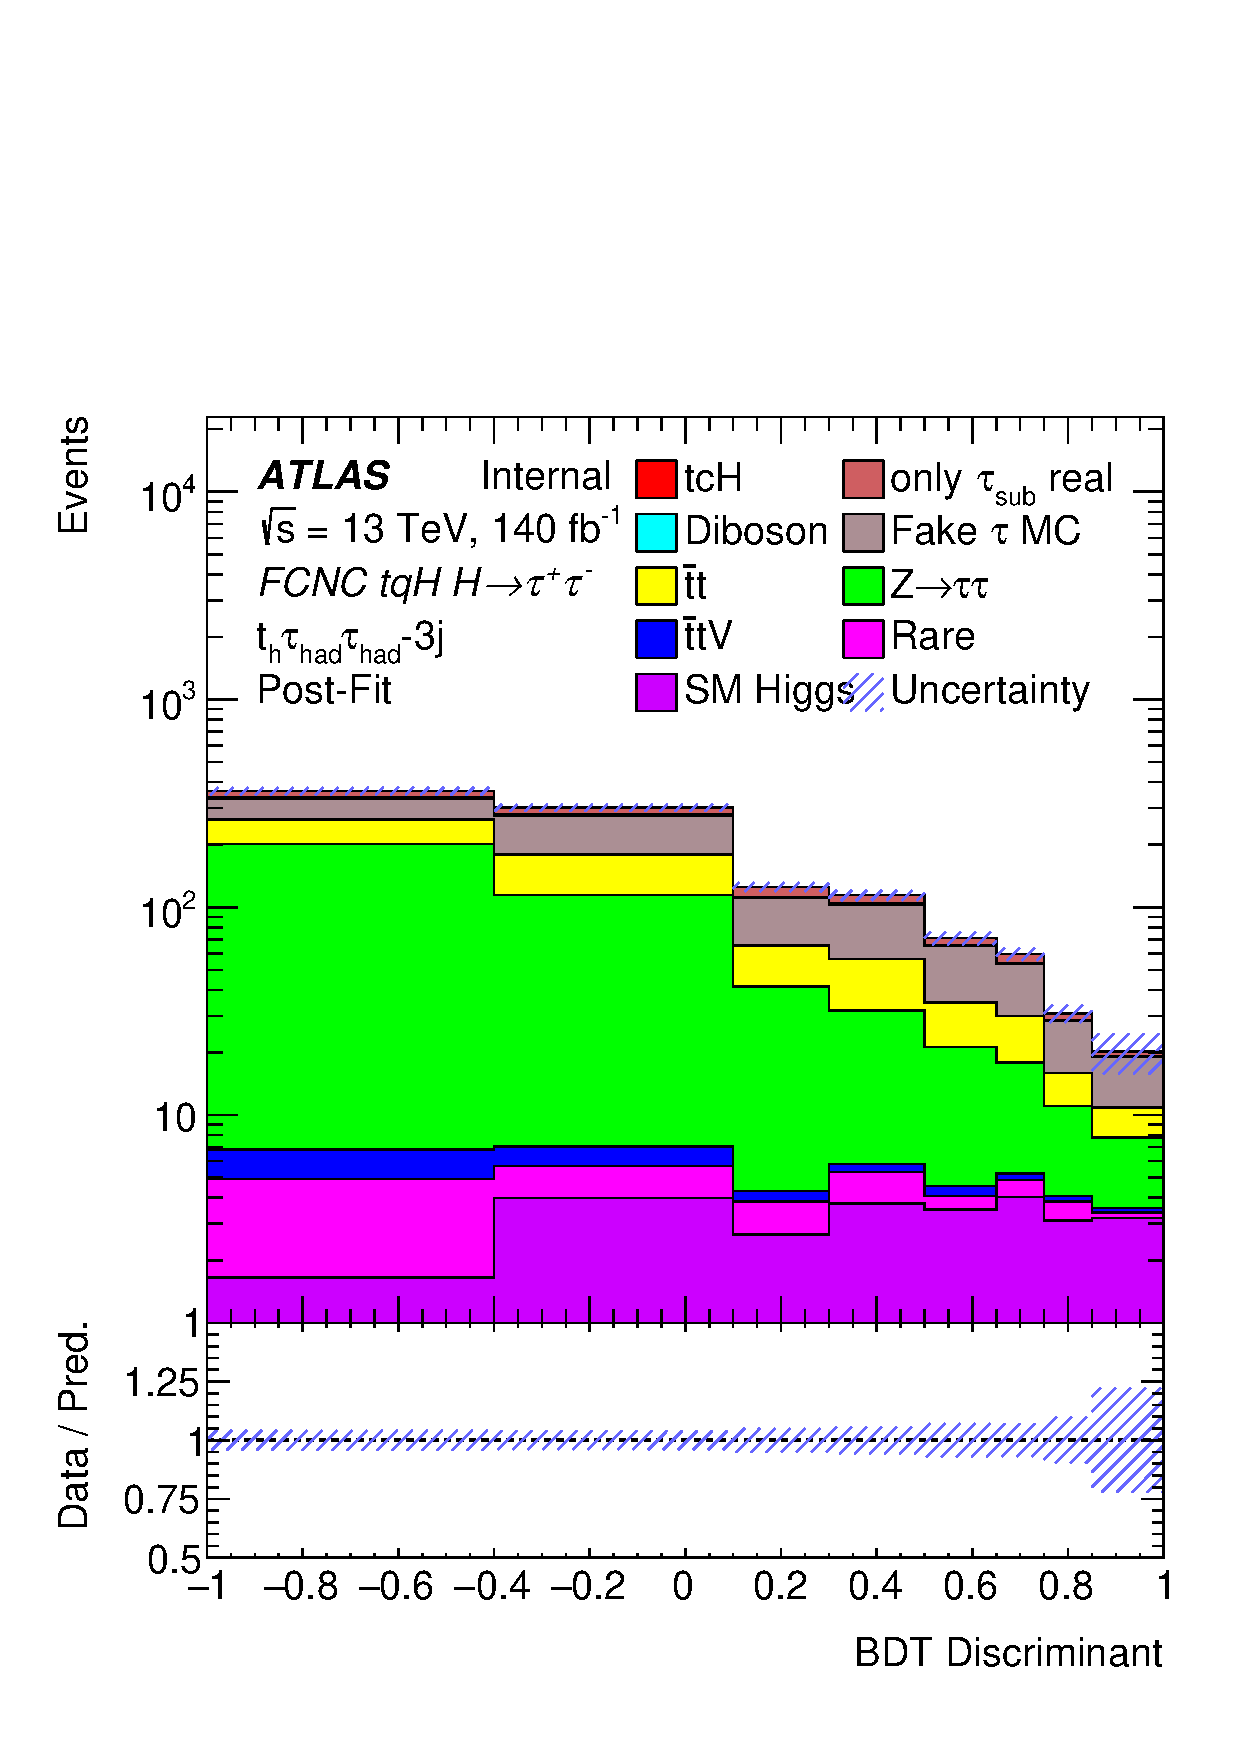
\includegraphics[width=0.30\textwidth]{\FCNCFigures/unblinded/xTFW/tcH_reg2mtau1b3jos_vetobtagwp70_highmet_postFit_BOnly.pdf}
\put(-100, 55){\textbf{(a3)}}\\
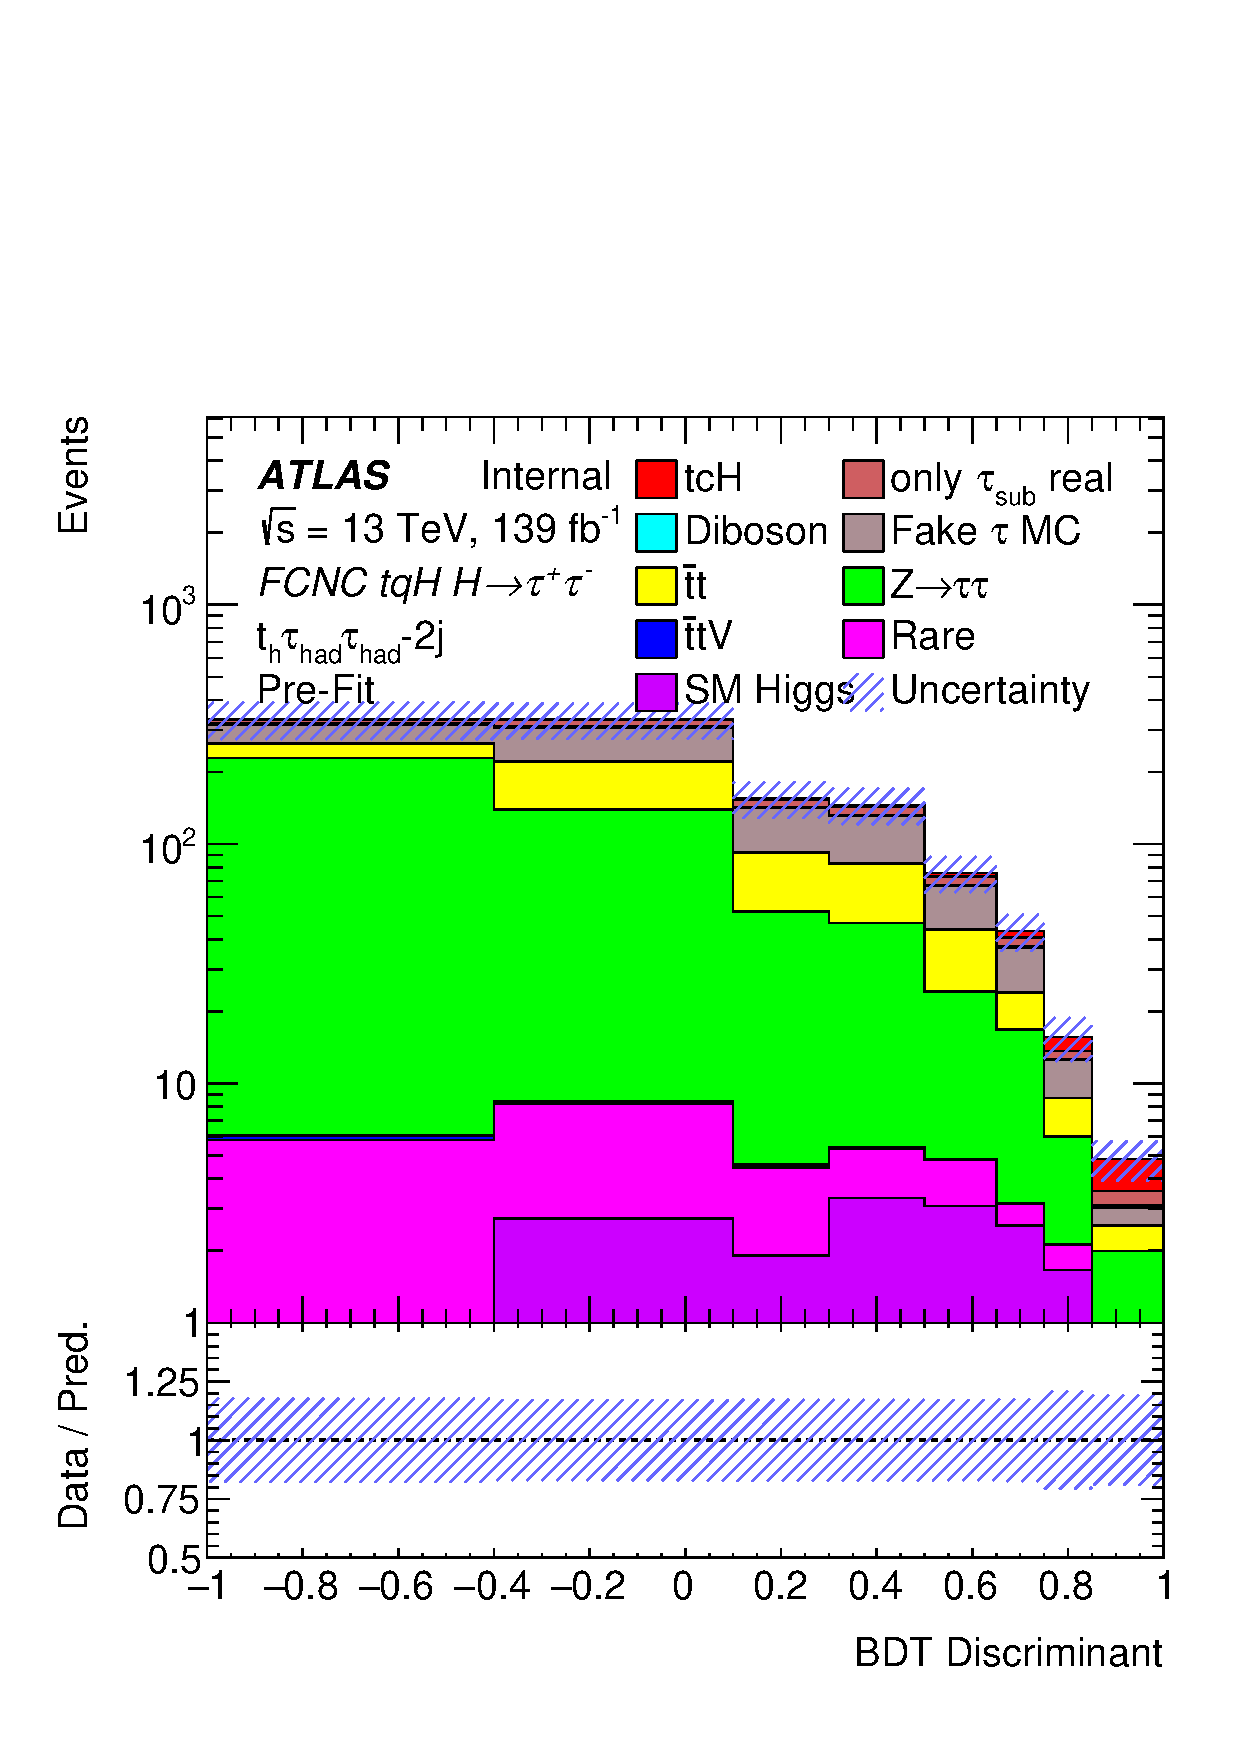
\includegraphics[width=0.30\textwidth]{\FCNCFigures/unblinded/xTFW/tcH_reg2mtau1b2jos_vetobtagwp70_highmet.pdf}
\put(-100, 55){\textbf{(b1)}}
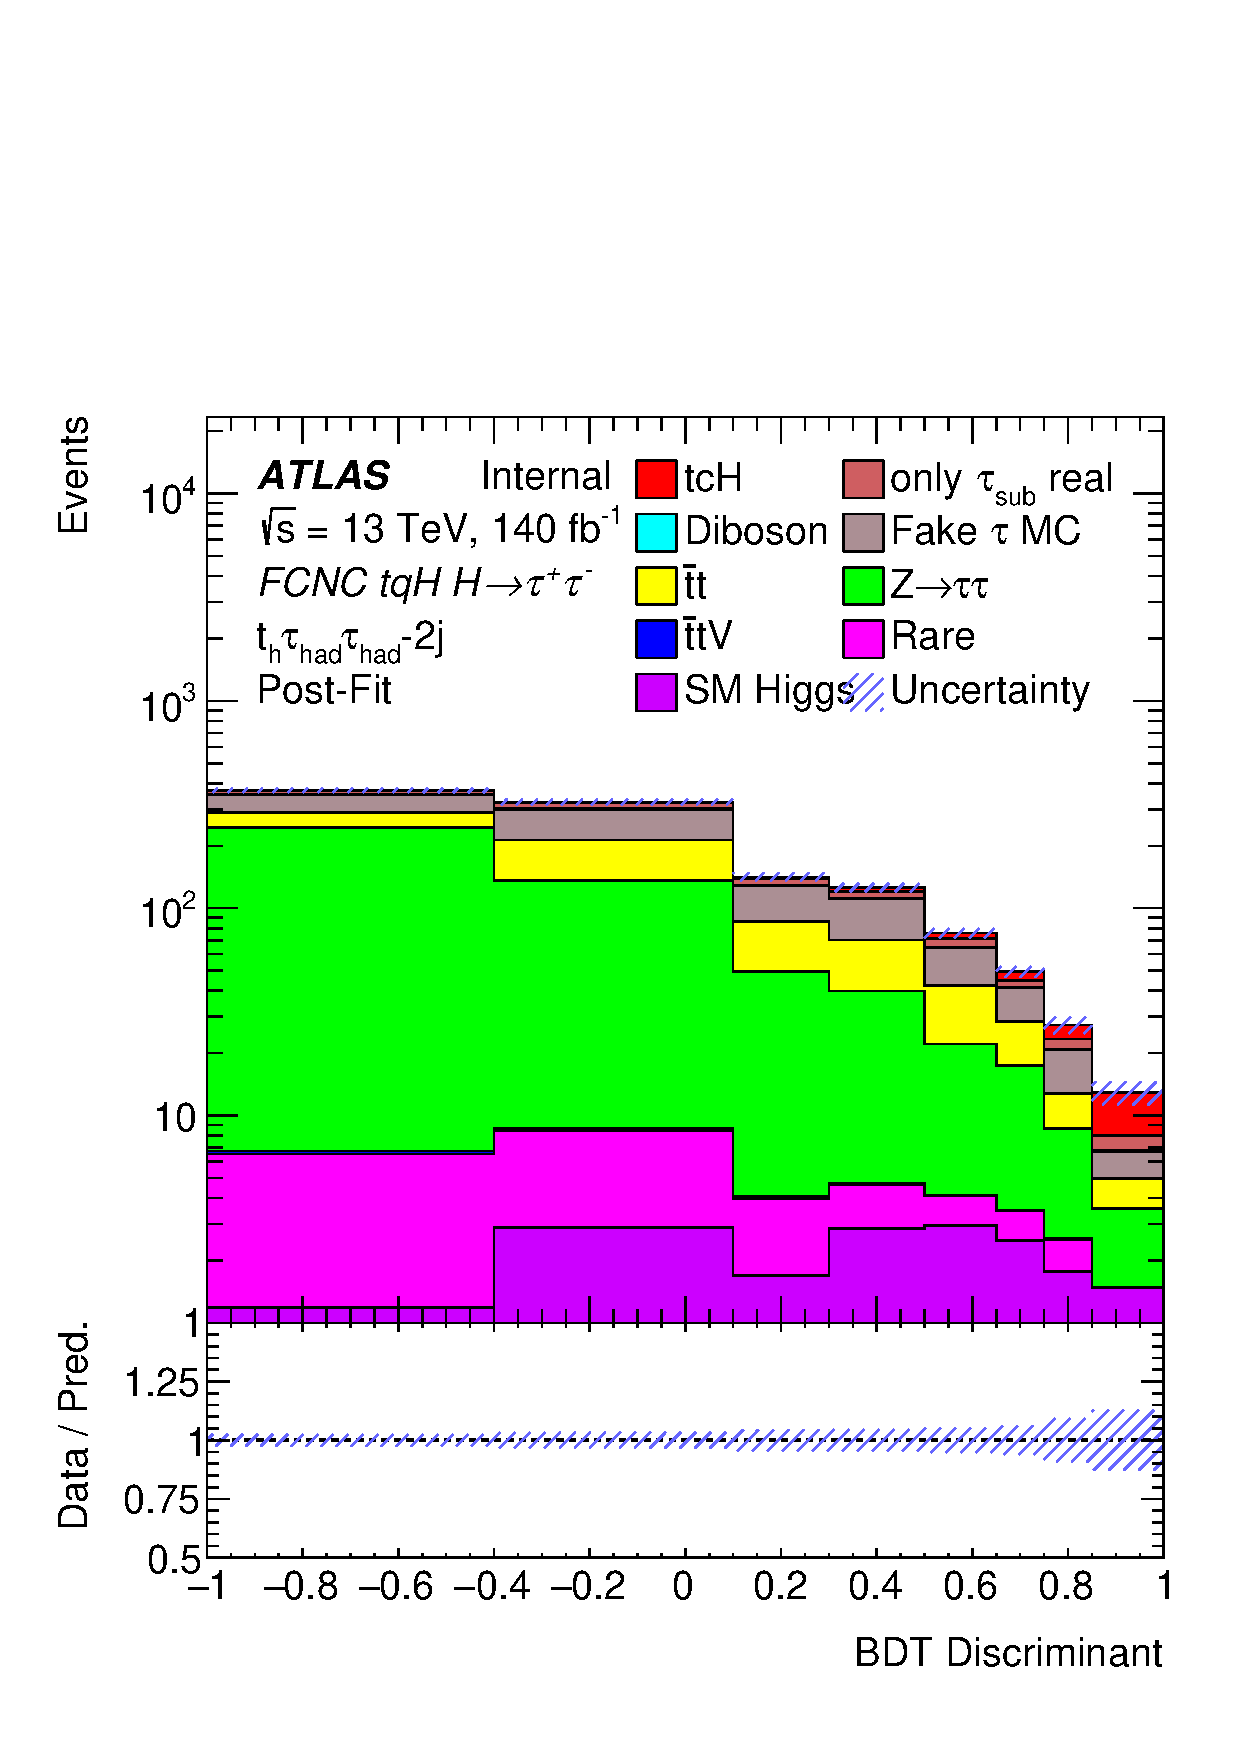
\includegraphics[width=0.30\textwidth]{\FCNCFigures/unblinded/xTFW/tcH_reg2mtau1b2jos_vetobtagwp70_highmet_postFit.pdf}
\put(-100, 55){\textbf{(b2)}}
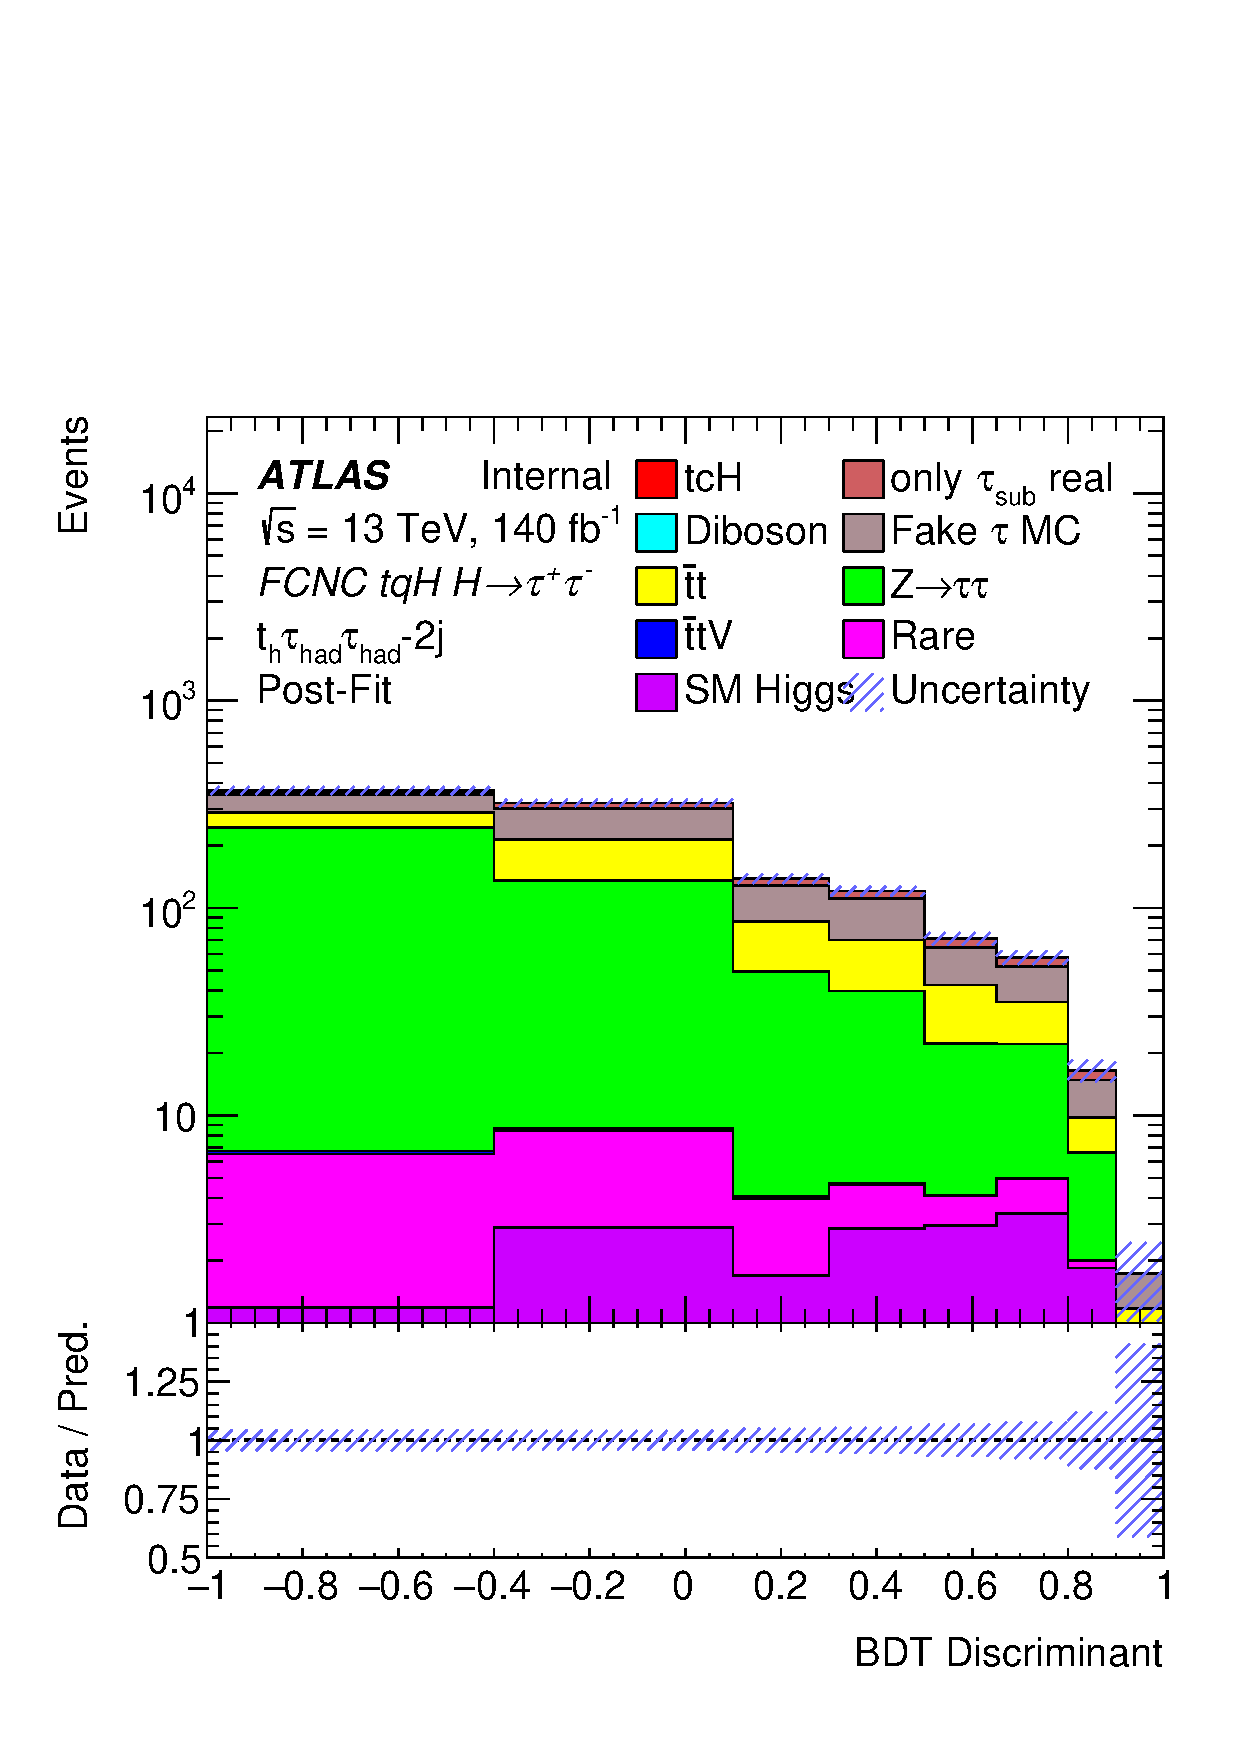
\includegraphics[width=0.30\textwidth]{\FCNCFigures/unblinded/xTFW/tcH_reg2mtau1b2jos_vetobtagwp70_highmet_postFit_BOnly.pdf}
\put(-100, 55){\textbf{(b3)}}\\

\caption{ Comparison of the shape of the BDT discriminant distribution between the unblinded prefit (a1,b1), unblinded postfit (a2,b2) and background only fit (a3,b3) in terms of tcH merged signal. The upper three plots are in the  $t_h\thadhad$-3j (a1-a3) region, and the bottom three are in $t_h\thadhad$-2j (b1-b3). Statistical and systematic uncertainties are being shown.}
\label{fig:xTFW_trexPrefit_tcH}
\end{figure}